\documentclass[11pt, a4paper]{article}\usepackage[]{graphicx}\usepackage[dvipsnames]{xcolor}
% maxwidth is the original width if it is less than linewidth
% otherwise use linewidth (to make sure the graphics do not exceed the margin)
\makeatletter
\def\maxwidth{ %
  \ifdim\Gin@nat@width>\linewidth
    \linewidth
  \else
    \Gin@nat@width
  \fi
}
\makeatother

\definecolor{fgcolor}{rgb}{0.345, 0.345, 0.345}
\newcommand{\hlnum}[1]{\textcolor[rgb]{0.686,0.059,0.569}{#1}}%
\newcommand{\hlstr}[1]{\textcolor[rgb]{0.192,0.494,0.8}{#1}}%
\newcommand{\hlcom}[1]{\textcolor[rgb]{0.678,0.584,0.686}{\textit{#1}}}%
\newcommand{\hlopt}[1]{\textcolor[rgb]{0,0,0}{#1}}%
\newcommand{\hlstd}[1]{\textcolor[rgb]{0.345,0.345,0.345}{#1}}%
\newcommand{\hlkwa}[1]{\textcolor[rgb]{0.161,0.373,0.58}{\textbf{#1}}}%
\newcommand{\hlkwb}[1]{\textcolor[rgb]{0.69,0.353,0.396}{#1}}%
\newcommand{\hlkwc}[1]{\textcolor[rgb]{0.333,0.667,0.333}{#1}}%
\newcommand{\hlkwd}[1]{\textcolor[rgb]{0.737,0.353,0.396}{\textbf{#1}}}%
\let\hlipl\hlkwb

\usepackage{framed}
\makeatletter
\newenvironment{kframe}{%
 \def\at@end@of@kframe{}%
 \ifinner\ifhmode%
  \def\at@end@of@kframe{\end{minipage}}%
  \begin{minipage}{\columnwidth}%
 \fi\fi%
 \def\FrameCommand##1{\hskip\@totalleftmargin \hskip-\fboxsep
 \colorbox{shadecolor}{##1}\hskip-\fboxsep
     % There is no \\@totalrightmargin, so:
     \hskip-\linewidth \hskip-\@totalleftmargin \hskip\columnwidth}%
 \MakeFramed {\advance\hsize-\width
   \@totalleftmargin\z@ \linewidth\hsize
   \@setminipage}}%
 {\par\unskip\endMakeFramed%
 \at@end@of@kframe}
\makeatother

\definecolor{shadecolor}{rgb}{.97, .97, .97}
\definecolor{messagecolor}{rgb}{0, 0, 0}
\definecolor{warningcolor}{rgb}{1, 0, 1}
\definecolor{errorcolor}{rgb}{1, 0, 0}
\newenvironment{knitrout}{}{} % an empty environment to be redefined in TeX

\usepackage{alltt}

\usepackage[top=1 in, bottom = 1 in, left = 1 in, right = 1 in ]{geometry}

\usepackage{amsmath, amssymb, amsfonts}
\usepackage{enumerate}
\usepackage[dvipsnames]{xcolor}  

\title{Two Factor Model : An Agricultural Example}
\author{Ananda Biswas}
\date{}
\IfFileExists{upquote.sty}{\usepackage{upquote}}{}
\begin{document}

\maketitle

Suppose in a hilly area, we have 24 plots. The plots are as identical as possible. 12 of them are in a plain region and rest 12 of them are in a tilted region. We have 3 varieties of a crop and we want to study their yields and how it is affected by slope. \\

\begin{figure}[h]
  \centering
  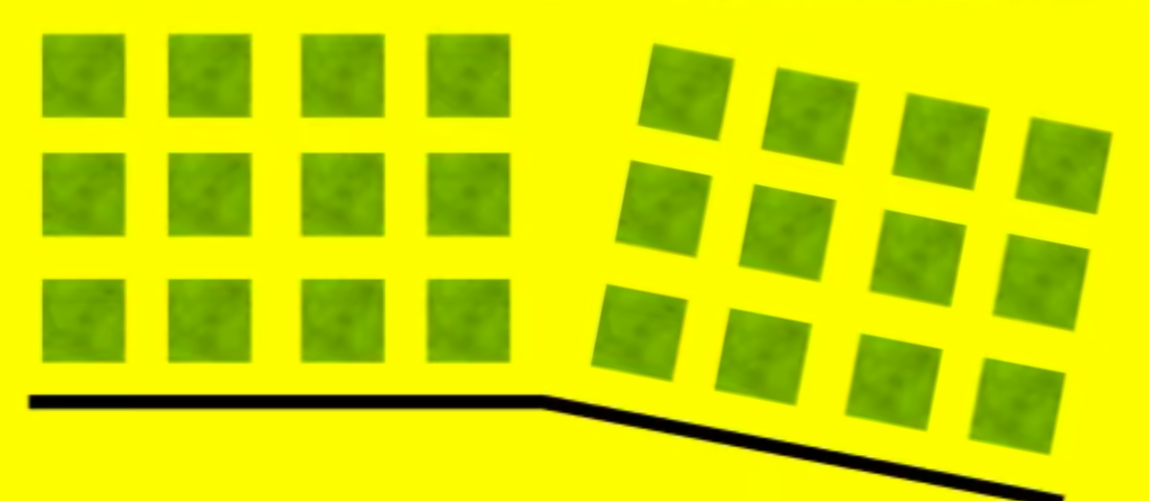
\includegraphics[scale = 0.5]{plots}
\end{figure}


Among the 12 plots in the plain region, we randomly select 4 plots and sow seeds of variety \textbf{1}, then we again randomly select another 4 plots and sow seeds of variety \textbf{2} and in the rest 4 plots we sow seeds of variety \textbf{3}. \\

We do the same thing for the 12 plots in tilted region. \\

The allocation of various varieties in the plots is as follows : \\

\begin{figure}[h]
  \centering
  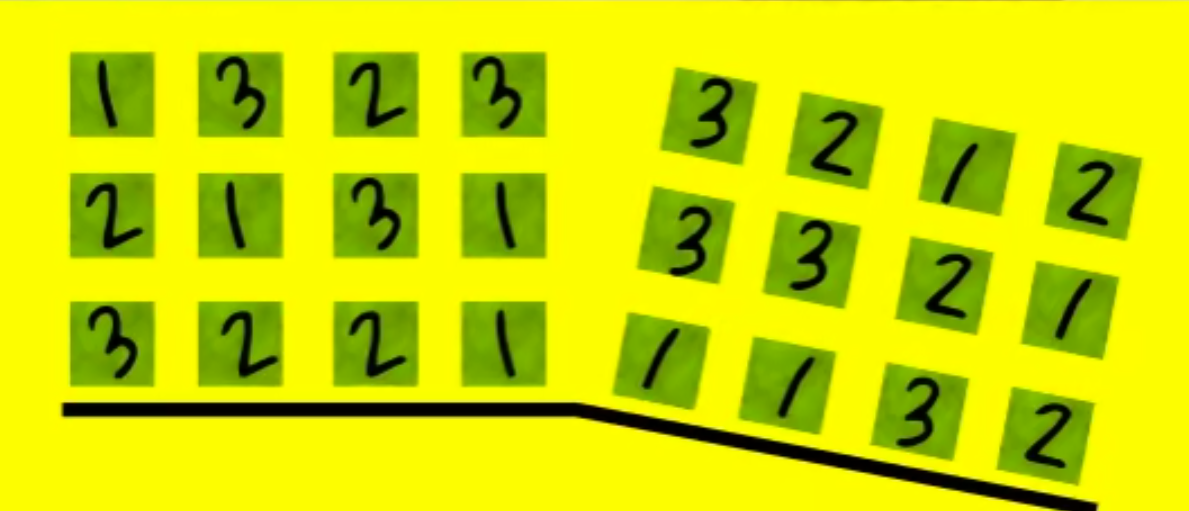
\includegraphics[scale = 0.5]{allocation}
\end{figure}

Here our blackbox diagram is : 

\begin{figure}[h]
  \centering
  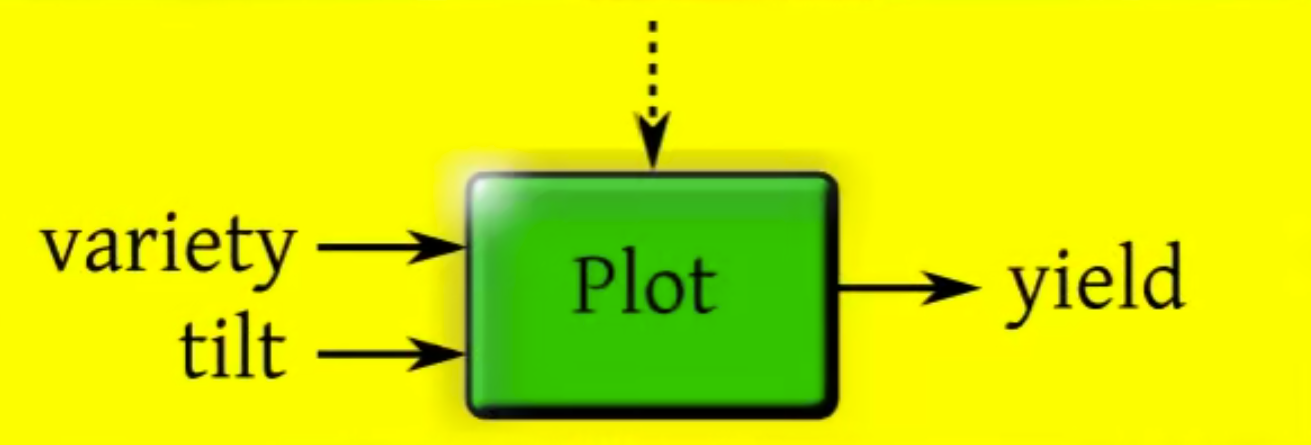
\includegraphics[scale = 0.5]{blackbox}
\end{figure}


Here our linear model will be : 

$$y_{ijk} = \alpha_i + \beta_j + \epsilon_{ijk}$$

where $\vec{\epsilon} \sim (\vec{0}, \sigma^2 I)$; \\

$i$ is the index for variety; \\

$j$ is the index for region (plane or tilted); \\

$k$ is the index for plot of certain variety in certain region. \\

Here $i = 1, 2, 3$, $j = 1, 2$ and $k = 1, 2, 3, 4$.

\section*{Two Factor Model without Interaction (Additive Model)}

Let us have a data set of yield of 3 varieties of paddy IR8, Jaya, Taichung in plain and slopy regions.

\begin{knitrout}
\definecolor{shadecolor}{rgb}{0.969, 0.969, 0.969}\color{fgcolor}\begin{kframe}
\begin{alltt}
\hlkwd{getwd}\hlstd{()}
\end{alltt}
\begin{verbatim}
## [1] "D:/Programming Languages/R/Linear Statistical Models - Arnab Chakraborty/005"
\end{verbatim}
\end{kframe}
\end{knitrout}

\begin{knitrout}
\definecolor{shadecolor}{rgb}{0.969, 0.969, 0.969}\color{fgcolor}\begin{kframe}
\begin{alltt}
\hlstd{agri_dat} \hlkwb{=} \hlkwd{read.csv}\hlstd{(}\hlstr{"agriculture_dataset.csv"}\hlstd{,} \hlkwc{as.is} \hlstd{=} \hlnum{FALSE}\hlstd{)}

\hlstd{agri_dat}
\end{alltt}
\begin{verbatim}
##     variety  tilt yield
## 1       IR8 plain 254.2
## 2       IR8 plain 253.9
## 3       IR8 plain 254.4
## 4       IR8 plain 254.2
## 5       IR8 plain 254.0
## 6       IR8 slope 261.0
## 7       IR8 slope 260.4
## 8       IR8 slope 261.1
## 9       IR8 slope 260.9
## 10      IR8 slope 261.1
## 11     Jaya plain 264.5
## 12     Jaya plain 264.7
## 13     Jaya plain 264.3
## 14     Jaya plain 264.2
## 15     Jaya plain 264.3
## 16     Jaya slope 270.7
## 17     Jaya slope 271.3
## 18     Jaya slope 270.6
## 19     Jaya slope 271.2
## 20     Jaya slope 270.7
## 21 Taichung plain 284.2
## 22 Taichung plain 284.6
## 23 Taichung plain 284.6
## 24 Taichung plain 285.0
## 25 Taichung plain 284.4
## 26 Taichung slope 291.1
## 27 Taichung slope 291.1
## 28 Taichung slope 291.2
## 29 Taichung slope 291.2
## 30 Taichung slope 291.5
\end{verbatim}
\begin{alltt}
\hlkwd{dim}\hlstd{(agri_dat)}
\end{alltt}
\begin{verbatim}
## [1] 30  3
\end{verbatim}
\begin{alltt}
\hlkwd{names}\hlstd{(agri_dat)}
\end{alltt}
\begin{verbatim}
## [1] "variety" "tilt"    "yield"
\end{verbatim}
\begin{alltt}
\hlkwd{head}\hlstd{(agri_dat)}
\end{alltt}
\begin{verbatim}
##   variety  tilt yield
## 1     IR8 plain 254.2
## 2     IR8 plain 253.9
## 3     IR8 plain 254.4
## 4     IR8 plain 254.2
## 5     IR8 plain 254.0
## 6     IR8 slope 261.0
\end{verbatim}
\begin{alltt}
\hlkwd{tail}\hlstd{(agri_dat)}
\end{alltt}
\begin{verbatim}
##     variety  tilt yield
## 25 Taichung plain 284.4
## 26 Taichung slope 291.1
## 27 Taichung slope 291.1
## 28 Taichung slope 291.2
## 29 Taichung slope 291.2
## 30 Taichung slope 291.5
\end{verbatim}
\end{kframe}
\end{knitrout}

Setting \textit{as.is = FALSE} tells R to read the strings in the csv file a factors, not characters.

\newpage

\begin{knitrout}
\definecolor{shadecolor}{rgb}{0.969, 0.969, 0.969}\color{fgcolor}\begin{kframe}
\begin{alltt}
\hlkwd{library}\hlstd{(tidyverse)}
\end{alltt}


{\ttfamily\noindent\color{warningcolor}{\#\# Warning: package 'tidyverse' was built under R version 4.2.3}}

{\ttfamily\noindent\color{warningcolor}{\#\# Warning: package 'ggplot2' was built under R version 4.2.2}}

{\ttfamily\noindent\color{warningcolor}{\#\# Warning: package 'tibble' was built under R version 4.2.3}}

{\ttfamily\noindent\color{warningcolor}{\#\# Warning: package 'tidyr' was built under R version 4.2.3}}

{\ttfamily\noindent\color{warningcolor}{\#\# Warning: package 'readr' was built under R version 4.2.2}}

{\ttfamily\noindent\color{warningcolor}{\#\# Warning: package 'purrr' was built under R version 4.2.3}}

{\ttfamily\noindent\color{warningcolor}{\#\# Warning: package 'dplyr' was built under R version 4.2.3}}

{\ttfamily\noindent\color{warningcolor}{\#\# Warning: package 'stringr' was built under R version 4.2.3}}

{\ttfamily\noindent\color{warningcolor}{\#\# Warning: package 'forcats' was built under R version 4.2.2}}

{\ttfamily\noindent\color{warningcolor}{\#\# Warning: package 'lubridate' was built under R version 4.2.2}}

{\ttfamily\noindent\itshape\color{messagecolor}{\#\# -- Attaching core tidyverse packages ------------------------ tidyverse 2.0.0 --\\\#\# v dplyr \ \ \ \ 1.1.3 \ \ \ \ v readr \ \ \ \ 2.1.4\\\#\# v forcats \ \ 1.0.0 \ \ \ \ v stringr \ \ 1.5.0\\\#\# v ggplot2 \ \ 3.4.1 \ \ \ \ v tibble \ \ \ 3.2.1\\\#\# v lubridate 1.9.2 \ \ \ \ v tidyr \ \ \ \ 1.3.0\\\#\# v purrr \ \ \ \ 1.0.2 \ \ \ \ \\\#\# -- Conflicts ------------------------------------------ tidyverse\_conflicts() --\\\#\# x dplyr::filter() masks stats::filter()\\\#\# x dplyr::lag() \ \ \ masks stats::lag()\\\#\# i Use the conflicted package (<http://conflicted.r-lib.org/>) to force all conflicts to become errors}}\end{kframe}
\end{knitrout}

\newpage

\begin{knitrout}
\definecolor{shadecolor}{rgb}{0.969, 0.969, 0.969}\color{fgcolor}\begin{kframe}
\begin{alltt}
\hlstd{agri_dat} \hlopt
  \hlkwd{ggplot}\hlstd{(}\hlkwd{aes}\hlstd{(}\hlkwc{x} \hlstd{= tilt,} \hlkwc{y} \hlstd{= yield))} \hlopt{+}
  \hlkwd{stat_boxplot}\hlstd{(}\hlkwc{geom} \hlstd{=} \hlstr{"errorbar"}\hlstd{,} \hlkwc{linewidth} \hlstd{=} \hlnum{1}\hlstd{)} \hlopt{+}
  \hlkwd{geom_boxplot}\hlstd{(}\hlkwc{fill} \hlstd{=} \hlstr{"#1BF248"}\hlstd{)} \hlopt{+}
  \hlkwd{labs}\hlstd{(}\hlkwc{x} \hlstd{=} \hlstr{"Tilt"}\hlstd{,} \hlkwc{y} \hlstd{=} \hlstr{"Yield"}\hlstd{,} \hlkwc{title} \hlstd{=} \hlstr{"Boxplot of Yield in Different Tilts"}\hlstd{)}
\end{alltt}
\end{kframe}
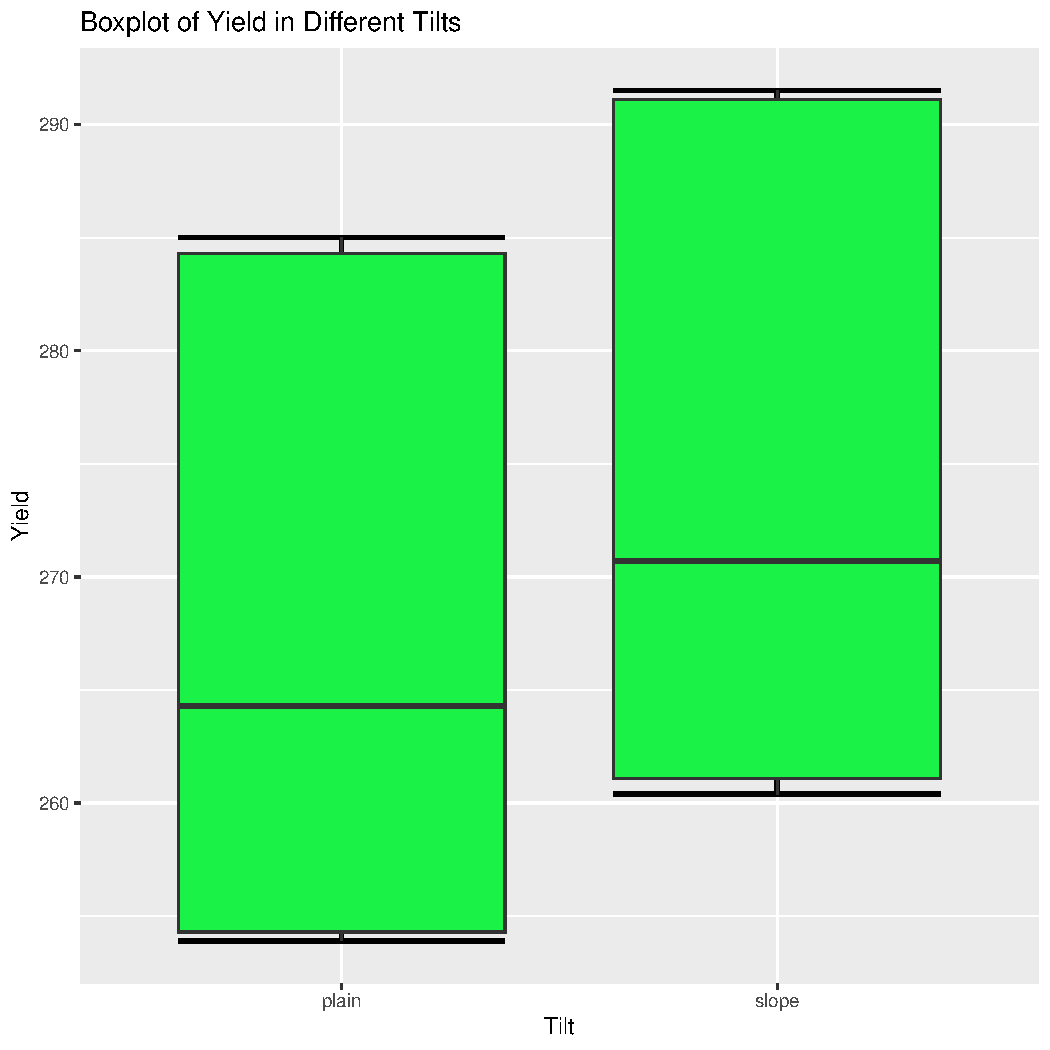
\includegraphics[width=\maxwidth]{figure/unnamed-chunk-4-1} 
\end{knitrout}

\newpage

\begin{knitrout}
\definecolor{shadecolor}{rgb}{0.969, 0.969, 0.969}\color{fgcolor}\begin{kframe}
\begin{alltt}
\hlstd{agri_dat} \hlopt
  \hlkwd{ggplot}\hlstd{(}\hlkwd{aes}\hlstd{(}\hlkwc{x} \hlstd{= variety,} \hlkwc{y} \hlstd{= yield))} \hlopt{+}
  \hlkwd{stat_boxplot}\hlstd{(}\hlkwc{geom} \hlstd{=} \hlstr{"errorbar"}\hlstd{,} \hlkwc{linewidth} \hlstd{=} \hlnum{1}\hlstd{)} \hlopt{+}
  \hlkwd{geom_boxplot}\hlstd{(}\hlkwc{fill} \hlstd{=} \hlstr{"#56DFEA"}\hlstd{)} \hlopt{+}
  \hlkwd{labs}\hlstd{(}\hlkwc{x} \hlstd{=} \hlstr{"Variety"}\hlstd{,} \hlkwc{y} \hlstd{=} \hlstr{"Yield"}\hlstd{,} \hlkwc{title} \hlstd{=} \hlstr{"Boxplot of Yield of Different Varieties"}\hlstd{)}
\end{alltt}
\end{kframe}
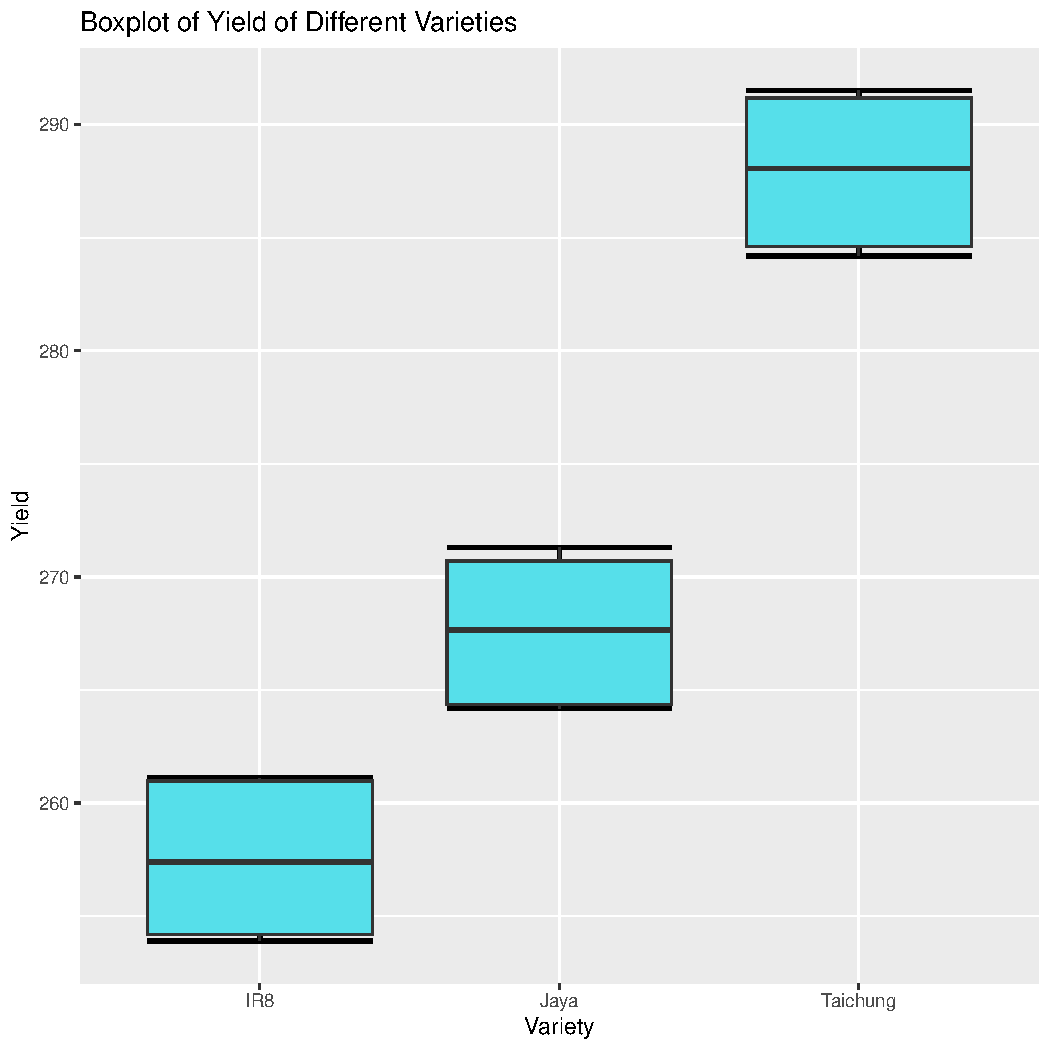
\includegraphics[width=\maxwidth]{figure/unnamed-chunk-5-1} 
\end{knitrout}

\newpage

\begin{knitrout}
\definecolor{shadecolor}{rgb}{0.969, 0.969, 0.969}\color{fgcolor}\begin{kframe}
\begin{alltt}
\hlkwd{with}\hlstd{(agri_dat,} \hlkwd{interaction.plot}\hlstd{(tilt, variety, yield))}
\end{alltt}
\end{kframe}
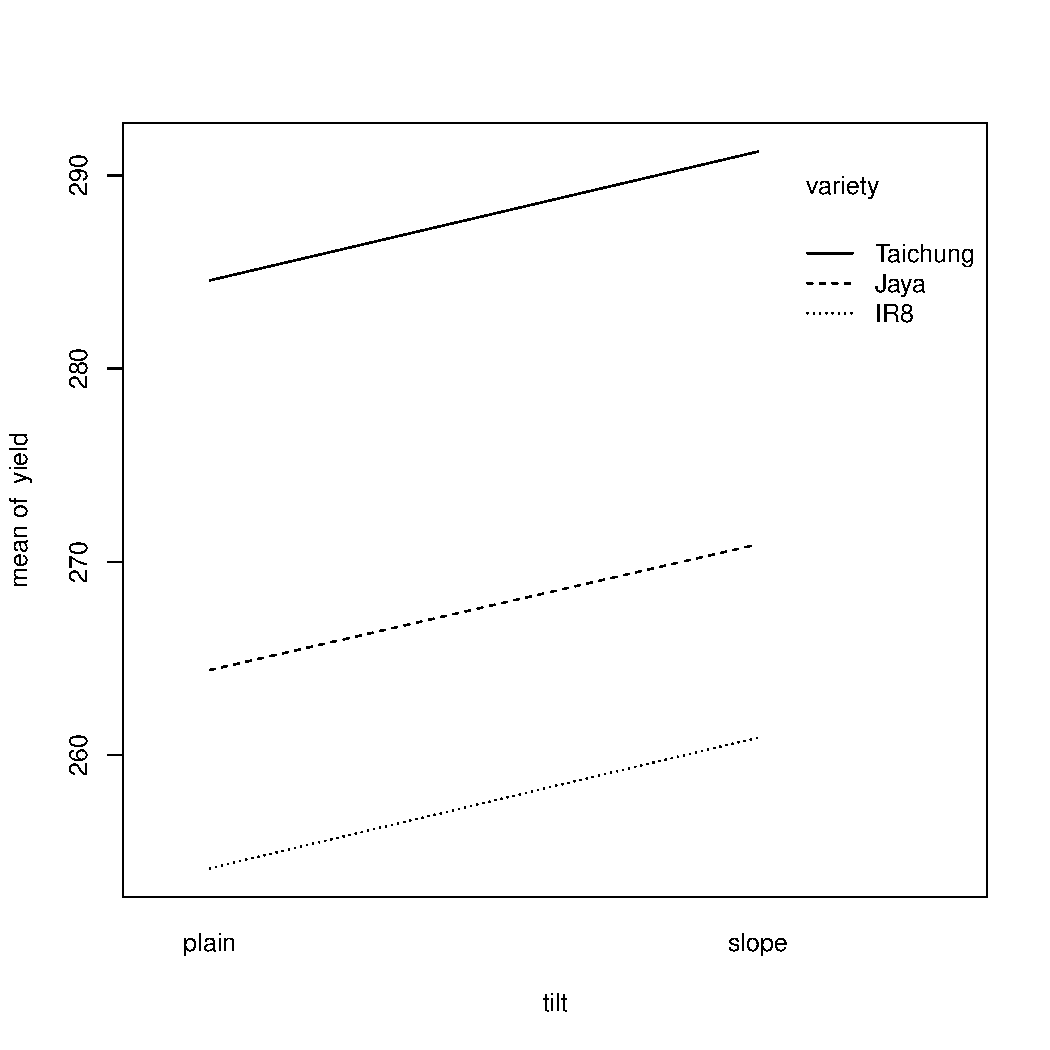
\includegraphics[width=\maxwidth]{figure/unnamed-chunk-6-1} 
\end{knitrout}

For interaction plot, the first argument is the variable that I want in x-axis, the second argument is the variable that I want as profile and the third argument is the variable that I want in y-axis.\\

\newpage

\begin{knitrout}
\definecolor{shadecolor}{rgb}{0.969, 0.969, 0.969}\color{fgcolor}\begin{kframe}
\begin{alltt}
\hlstd{df1} \hlkwb{<-} \hlstd{agri_dat} \hlopt
  \hlkwd{group_by}\hlstd{(variety, tilt)} \hlopt
  \hlkwd{summarise}\hlstd{(}\hlkwc{mean_yield} \hlstd{=} \hlkwd{mean}\hlstd{(yield))}
\end{alltt}


{\ttfamily\noindent\itshape\color{messagecolor}{\#\# `summarise()` has grouped output by 'variety'. You can override using the\\\#\# `.groups` argument.}}\begin{alltt}
\hlstd{df1} \hlopt
  \hlkwd{ggplot}\hlstd{(}\hlkwd{aes}\hlstd{(}\hlkwc{x} \hlstd{= tilt,} \hlkwc{y} \hlstd{= mean_yield))} \hlopt{+}
  \hlkwd{geom_line}\hlstd{(}\hlkwd{aes}\hlstd{(}\hlkwc{group} \hlstd{= variety,} \hlkwc{color} \hlstd{= variety),} \hlkwc{linewidth} \hlstd{=} \hlnum{1.5}\hlstd{)} \hlopt{+}
  \hlkwd{geom_point}\hlstd{(}\hlkwd{aes}\hlstd{(}\hlkwc{color} \hlstd{= variety),} \hlkwc{size} \hlstd{=} \hlnum{4}\hlstd{)} \hlopt{+}
  \hlkwd{labs}\hlstd{(}\hlkwc{x} \hlstd{=} \hlstr{"Tilt"}\hlstd{,} \hlkwc{y} \hlstd{=} \hlstr{"Mean Yield"}\hlstd{,} \hlkwc{title} \hlstd{=} \hlstr{"Interaction Plot of Different Varieties"}\hlstd{)}
\end{alltt}
\end{kframe}
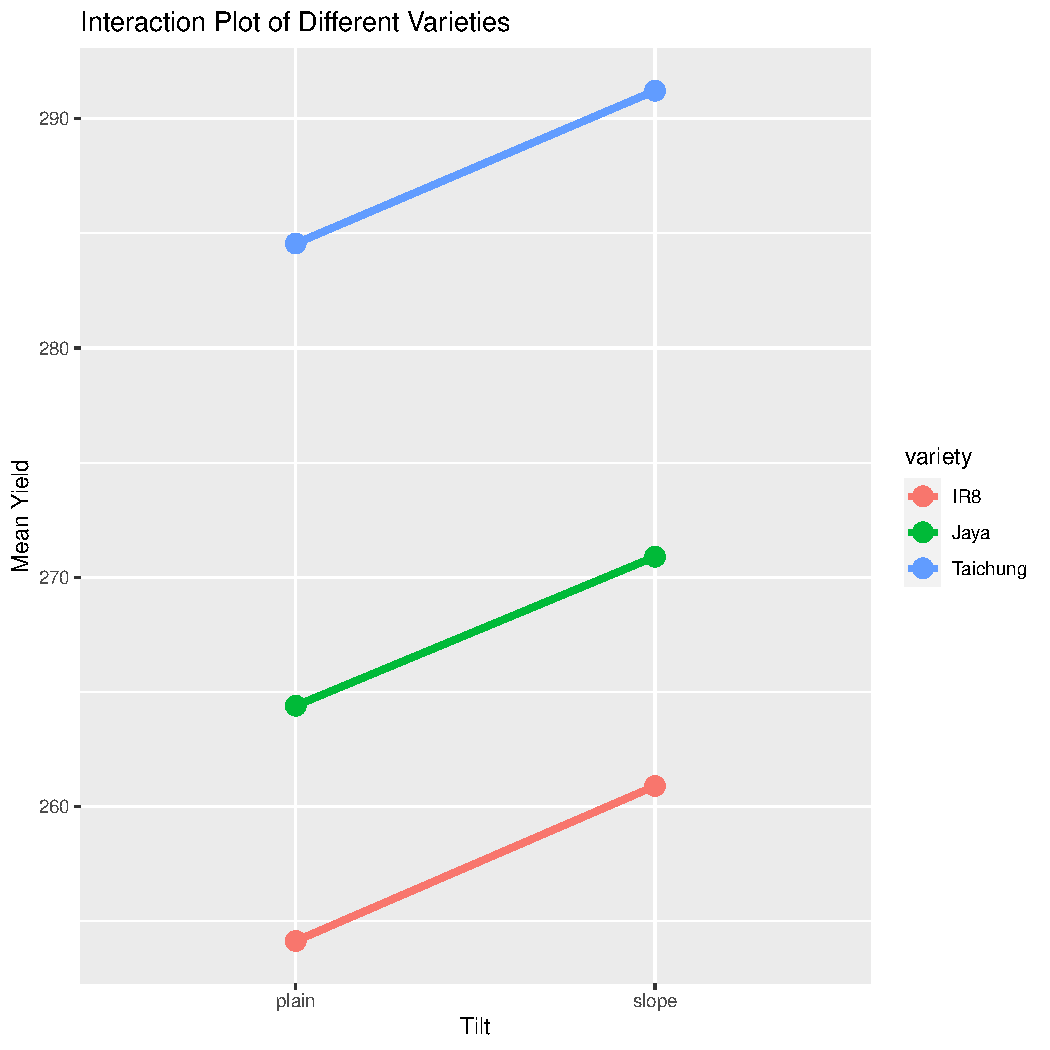
\includegraphics[width=\maxwidth]{figure/unnamed-chunk-7-1} 
\end{knitrout}

Such an interaction plot translates to an additive model.

The different varieties IR8, Jaya, Taichung are often referred as \textit{profiles}. \\

The boxplots verify that the homoscedasticity assumption is true.

\begin{knitrout}
\definecolor{shadecolor}{rgb}{0.969, 0.969, 0.969}\color{fgcolor}\begin{kframe}
\begin{alltt}
\hlstd{fit1} \hlkwb{=} \hlkwd{lm}\hlstd{(yield} \hlopt{~} \hlstd{tilt} \hlopt{+} \hlstd{variety,} \hlkwc{data} \hlstd{= agri_dat)}
\end{alltt}
\end{kframe}
\end{knitrout}

\begin{knitrout}
\definecolor{shadecolor}{rgb}{0.969, 0.969, 0.969}\color{fgcolor}\begin{kframe}
\begin{alltt}
\hlstd{fit1}
\end{alltt}
\begin{verbatim}
## 
## Call:
## lm(formula = yield ~ tilt + variety, data = agri_dat)
## 
## Coefficients:
##     (Intercept)        tiltslope      varietyJaya  varietyTaichung  
##          254.20             6.64            10.13            30.37
\end{verbatim}
\end{kframe}
\end{knitrout}

Here the linear model is :

$$y_{ijk} = \mu + \alpha_i + \beta_j + \epsilon_{ijk}$$

where $\mu$ is the benchmark yield. \\

The estimates of \textit{tiltplane} and \textit{varietyIR8} have been forced to 0; \textit{i.e.} 
$\alpha_1 = 0$ and $\beta_1 = 0$.

\begin{knitrout}
\definecolor{shadecolor}{rgb}{0.969, 0.969, 0.969}\color{fgcolor}\begin{kframe}
\begin{alltt}
\hlkwd{summary}\hlstd{(fit1)}
\end{alltt}
\begin{verbatim}
## 
## Call:
## lm(formula = yield ~ tilt + variety, data = agri_dat)
## 
## Residuals:
##     Min      1Q  Median      3Q     Max 
## -0.4400 -0.1600 -0.0050  0.1925  0.4300 
## 
## Coefficients:
##                  Estimate Std. Error t value Pr(>|t|)    
## (Intercept)     254.20000    0.09109 2790.64   <2e-16 ***
## tiltslope         6.64000    0.09109   72.89   <2e-16 ***
## varietyJaya      10.13000    0.11156   90.80   <2e-16 ***
## varietyTaichung  30.37000    0.11156  272.23   <2e-16 ***
## ---
## Signif. codes:  0 '***' 0.001 '**' 0.01 '*' 0.05 '.' 0.1 ' ' 1
## 
## Residual standard error: 0.2495 on 26 degrees of freedom
## Multiple R-squared:  0.9997,	Adjusted R-squared:  0.9996 
## F-statistic: 2.739e+04 on 3 and 26 DF,  p-value: < 2.2e-16
\end{verbatim}
\end{kframe}
\end{knitrout}

\begin{knitrout}
\definecolor{shadecolor}{rgb}{0.969, 0.969, 0.969}\color{fgcolor}\begin{kframe}
\begin{alltt}
\hlkwd{model.matrix}\hlstd{(fit1)}
\end{alltt}
\begin{verbatim}
##    (Intercept) tiltslope varietyJaya varietyTaichung
## 1            1         0           0               0
## 2            1         0           0               0
## 3            1         0           0               0
## 4            1         0           0               0
## 5            1         0           0               0
## 6            1         1           0               0
## 7            1         1           0               0
## 8            1         1           0               0
## 9            1         1           0               0
## 10           1         1           0               0
## 11           1         0           1               0
## 12           1         0           1               0
## 13           1         0           1               0
## 14           1         0           1               0
## 15           1         0           1               0
## 16           1         1           1               0
## 17           1         1           1               0
## 18           1         1           1               0
## 19           1         1           1               0
## 20           1         1           1               0
## 21           1         0           0               1
## 22           1         0           0               1
## 23           1         0           0               1
## 24           1         0           0               1
## 25           1         0           0               1
## 26           1         1           0               1
## 27           1         1           0               1
## 28           1         1           0               1
## 29           1         1           0               1
## 30           1         1           0               1
## attr(,"assign")
## [1] 0 1 2 2
## attr(,"contrasts")
## attr(,"contrasts")$tilt
## [1] "contr.treatment"
## 
## attr(,"contrasts")$variety
## [1] "contr.treatment"
\end{verbatim}
\end{kframe}
\end{knitrout}

\begin{knitrout}
\definecolor{shadecolor}{rgb}{0.969, 0.969, 0.969}\color{fgcolor}\begin{kframe}
\begin{alltt}
\hlstd{fit1}\hlopt{$}\hlstd{rank}
\end{alltt}
\begin{verbatim}
## [1] 4
\end{verbatim}
\end{kframe}
\end{knitrout}

\newpage

\begin{knitrout}
\definecolor{shadecolor}{rgb}{0.969, 0.969, 0.969}\color{fgcolor}\begin{kframe}
\begin{alltt}
\hlstd{temp_df} \hlkwb{<-} \hlkwd{data.frame}\hlstd{(fit1}\hlopt{$}\hlstd{residuals)}

\hlstd{temp_df} \hlopt
  \hlkwd{ggplot}\hlstd{(}\hlkwd{aes}\hlstd{(}\hlkwc{y} \hlstd{= fit1.residuals,} \hlkwc{x} \hlstd{=} \hlnum{1}\hlopt{:}\hlkwd{length}\hlstd{(fit1.residuals)))} \hlopt{+}
  \hlkwd{geom_point}\hlstd{(}\hlkwc{color} \hlstd{=} \hlstr{"red"}\hlstd{,} \hlkwc{size} \hlstd{=} \hlnum{3}\hlstd{)} \hlopt{+}
  \hlkwd{geom_hline}\hlstd{(}\hlkwc{yintercept} \hlstd{=} \hlnum{0}\hlstd{,} \hlkwc{color} \hlstd{=} \hlstr{"blue"}\hlstd{,} \hlkwc{linewidth} \hlstd{=} \hlnum{1}\hlstd{)} \hlopt{+}
  \hlkwd{labs}\hlstd{(}\hlkwc{x} \hlstd{=} \hlstr{"Index"}\hlstd{,} \hlkwc{y} \hlstd{=} \hlstr{"Residuals"}\hlstd{,} \hlkwc{title} \hlstd{=} \hlstr{"Residuals of fit1"}\hlstd{)}
\end{alltt}
\end{kframe}
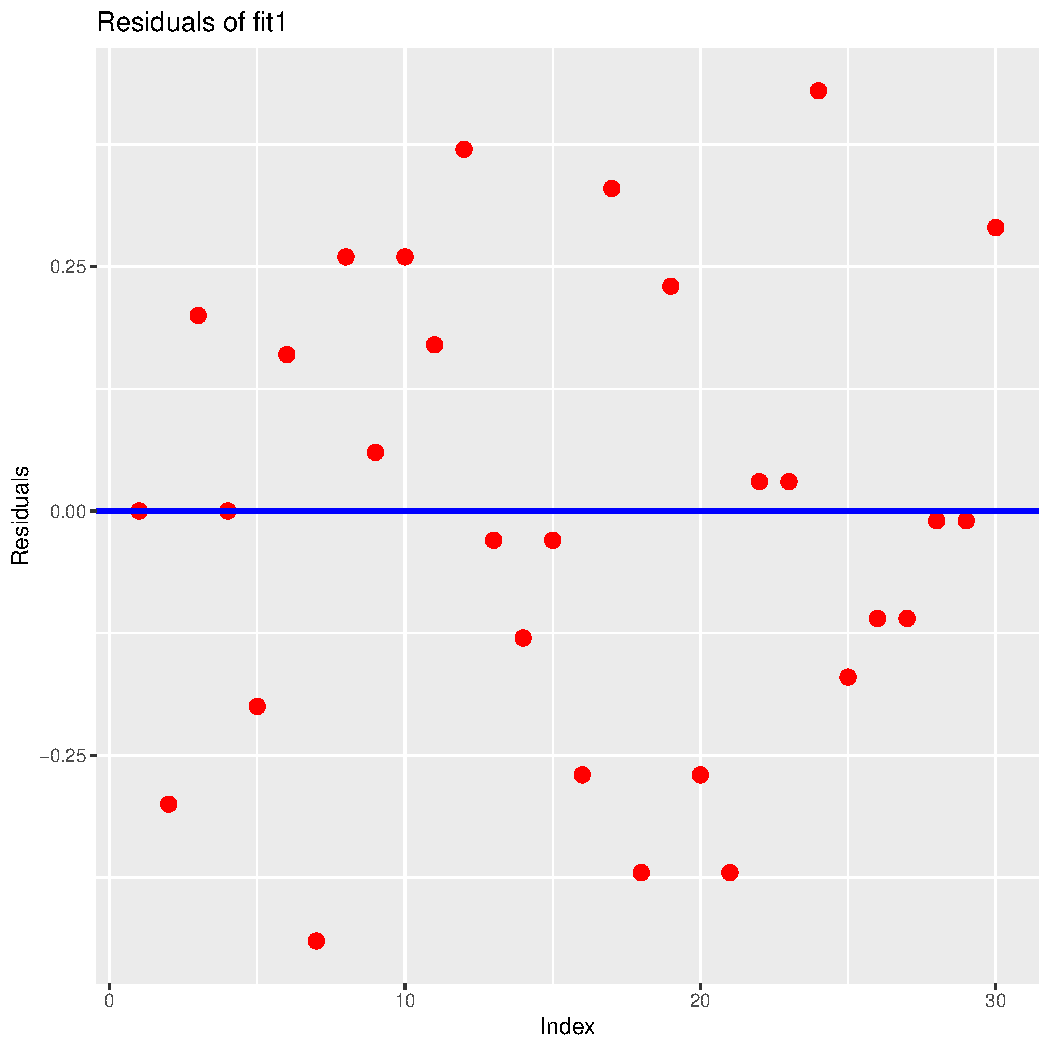
\includegraphics[width=\maxwidth]{figure/unnamed-chunk-13-1} 
\end{knitrout}

\newpage

\section*{Two Factor Model with Interaction}

\begin{figure}[h]
  \centering
  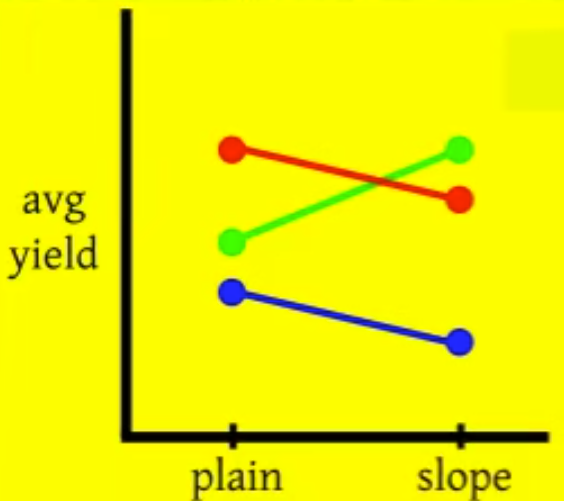
\includegraphics[scale = 0.4]{interaction_plot}
\end{figure}

If we have an interaction plot like the above \textit{i.e.} at least two of the profiles are intersecting or not so parallel, we shall introduce a new linear model where we shall take count of the interaction of the two factors. \\

The linear model is :

$$y_{ijk} = \mu + \alpha_i + \beta_j + \textcolor{red}{\gamma_{ij}} +  \epsilon_{ijk}$$

where $\textcolor{red}{\gamma_{ij}}$s take count of the interaction. \\

In practice, we shall first consider this model. We shall test whether $\gamma_{ij}$s are 0 or not. If all the $\gamma_{ij}$s are 0, then we shall resort to the \textbf{additive model}. If any one of the $\gamma_{ij}$s is non-zero, then we shall report that. But we shall never estimate $\gamma_{ij}$s. \\

For a statistician, interaction is bad news. Because, when there is no interaction, we can talk about the inputs separately. But interaction spoils the fun by saying, you cannot really say how the inputs are connected to the output, they are inextricable; and it is their combined influence which is effecting the output. So all that a statistician can say is \textit{things are twisted} and nothing more. \\

$\bullet$ \textbf{Cell Means Model} \\

When we find any one of the $\gamma_{ij}$s is non-zero (\textit{i.e.} there is some interaction), then we shall resort to this model :

$$y_{ijk} = \mu_{ij} + \epsilon_{ijk}$$

where $\mu_{ij}$ is the expected yield of variety $i$ in tilt $j$ and the fluctuations in $y_{ijk}$ are due to the random error $\epsilon_{ijk}$.

\begin{knitrout}
\definecolor{shadecolor}{rgb}{0.969, 0.969, 0.969}\color{fgcolor}\begin{kframe}
\begin{alltt}
\hlkwd{getwd}\hlstd{()}
\end{alltt}
\begin{verbatim}
## [1] "D:/Programming Languages/R/Linear Statistical Models - Arnab Chakraborty/005"
\end{verbatim}
\end{kframe}
\end{knitrout}

\begin{knitrout}
\definecolor{shadecolor}{rgb}{0.969, 0.969, 0.969}\color{fgcolor}\begin{kframe}
\begin{alltt}
\hlstd{paddy_data} \hlkwb{=} \hlkwd{read.csv}\hlstd{(}\hlstr{"agriculture_dataset_2.csv"}\hlstd{)}

\hlstd{paddy_data}
\end{alltt}
\begin{verbatim}
##     variety  tilt  yield
## 1       IR8 plain 250.20
## 2       IR8 plain 249.97
## 3       IR8 plain 250.08
## 4       IR8 plain 250.29
## 5       IR8 plain 250.27
## 6       IR8 slope 240.50
## 7       IR8 slope 240.82
## 8       IR8 slope 240.61
## 9       IR8 slope 240.30
## 10      IR8 slope 240.65
## 11     Jaya plain 260.75
## 12     Jaya plain 260.64
## 13     Jaya plain 260.57
## 14     Jaya plain 260.17
## 15     Jaya plain 260.52
## 16     Jaya slope 275.32
## 17     Jaya slope 275.56
## 18     Jaya slope 275.59
## 19     Jaya slope 275.24
## 20     Jaya slope 275.82
## 21 Taichung plain 280.76
## 22 Taichung plain 280.83
## 23 Taichung plain 281.29
## 24 Taichung plain 280.66
## 25 Taichung plain 280.62
## 26 Taichung slope 252.79
## 27 Taichung slope 252.92
## 28 Taichung slope 253.29
## 29 Taichung slope 253.25
## 30 Taichung slope 253.14
\end{verbatim}
\begin{alltt}
\hlkwd{dim}\hlstd{(paddy_data)}
\end{alltt}
\begin{verbatim}
## [1] 30  3
\end{verbatim}
\begin{alltt}
\hlkwd{names}\hlstd{(paddy_data)}
\end{alltt}
\begin{verbatim}
## [1] "variety" "tilt"    "yield"
\end{verbatim}
\begin{alltt}
\hlkwd{head}\hlstd{(paddy_data)}
\end{alltt}
\begin{verbatim}
##   variety  tilt  yield
## 1     IR8 plain 250.20
## 2     IR8 plain 249.97
## 3     IR8 plain 250.08
## 4     IR8 plain 250.29
## 5     IR8 plain 250.27
## 6     IR8 slope 240.50
\end{verbatim}
\begin{alltt}
\hlkwd{tail}\hlstd{(paddy_data)}
\end{alltt}
\begin{verbatim}
##     variety  tilt  yield
## 25 Taichung plain 280.62
## 26 Taichung slope 252.79
## 27 Taichung slope 252.92
## 28 Taichung slope 253.29
## 29 Taichung slope 253.25
## 30 Taichung slope 253.14
\end{verbatim}
\end{kframe}
\end{knitrout}

\newpage

\begin{knitrout}
\definecolor{shadecolor}{rgb}{0.969, 0.969, 0.969}\color{fgcolor}\begin{kframe}
\begin{alltt}
\hlkwd{with}\hlstd{(}\hlkwc{data} \hlstd{= paddy_data,} \hlkwd{boxplot}\hlstd{(yield} \hlopt{~} \hlstd{variety}\hlopt{:}\hlstd{tilt))}
\end{alltt}
\end{kframe}
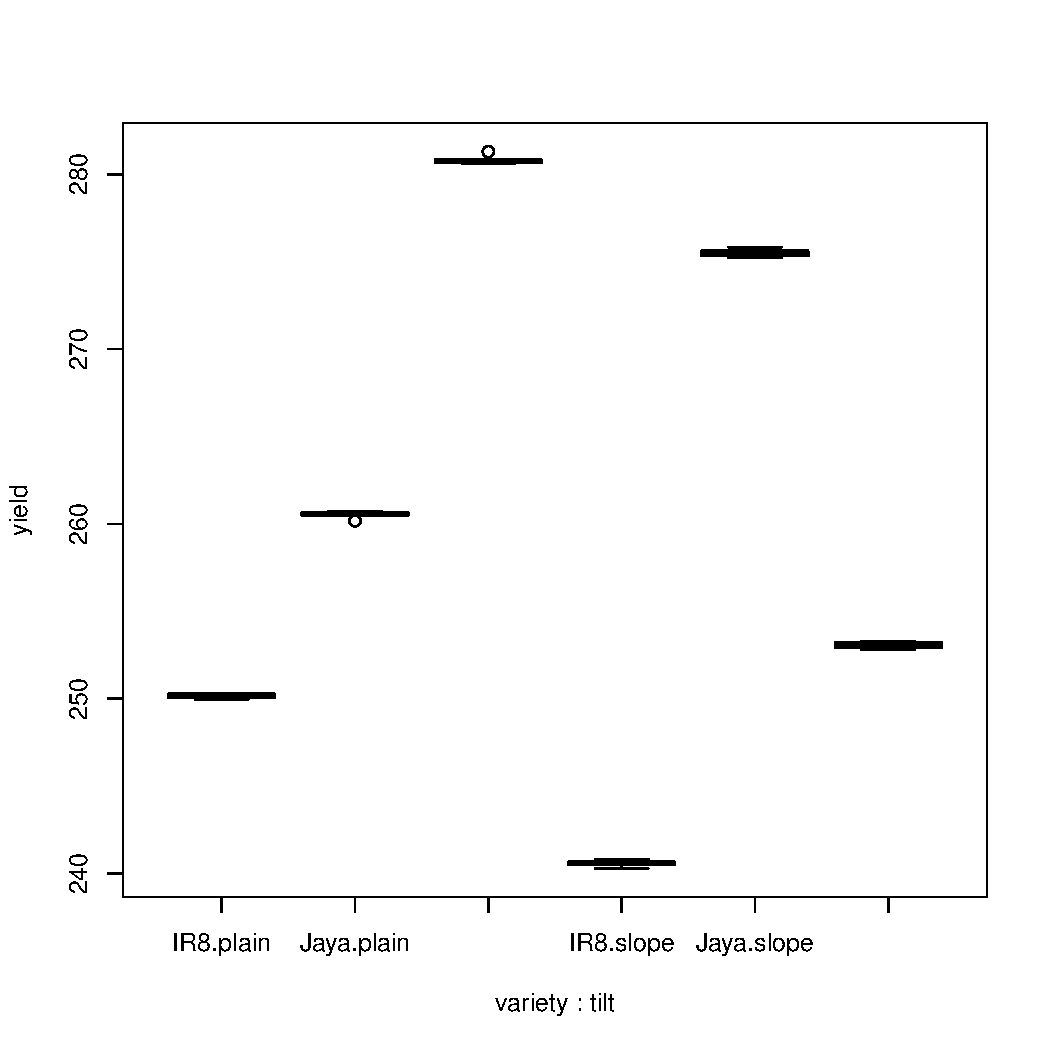
\includegraphics[width=\maxwidth]{figure/unnamed-chunk-16-1} 
\end{knitrout}

\newpage

\begin{knitrout}
\definecolor{shadecolor}{rgb}{0.969, 0.969, 0.969}\color{fgcolor}\begin{kframe}
\begin{alltt}
\hlstd{paddy_data} \hlopt
  \hlkwd{ggplot}\hlstd{(}\hlkwd{aes}\hlstd{(}\hlkwc{x} \hlstd{=} \hlkwd{interaction}\hlstd{(variety, tilt),} \hlkwc{y} \hlstd{= yield))} \hlopt{+}
  \hlkwd{geom_boxplot}\hlstd{(}\hlkwc{col} \hlstd{=} \hlstr{"#0354F6"}\hlstd{)} \hlopt{+}
  \hlkwd{labs}\hlstd{(}\hlkwc{x} \hlstd{=} \hlstr{"Variety.Tilt"}\hlstd{,} \hlkwc{y} \hlstd{=} \hlstr{"Yield"}\hlstd{,} \hlkwc{title} \hlstd{=} \hlstr{"Boxplot of Different Yields"}\hlstd{)}
\end{alltt}
\end{kframe}
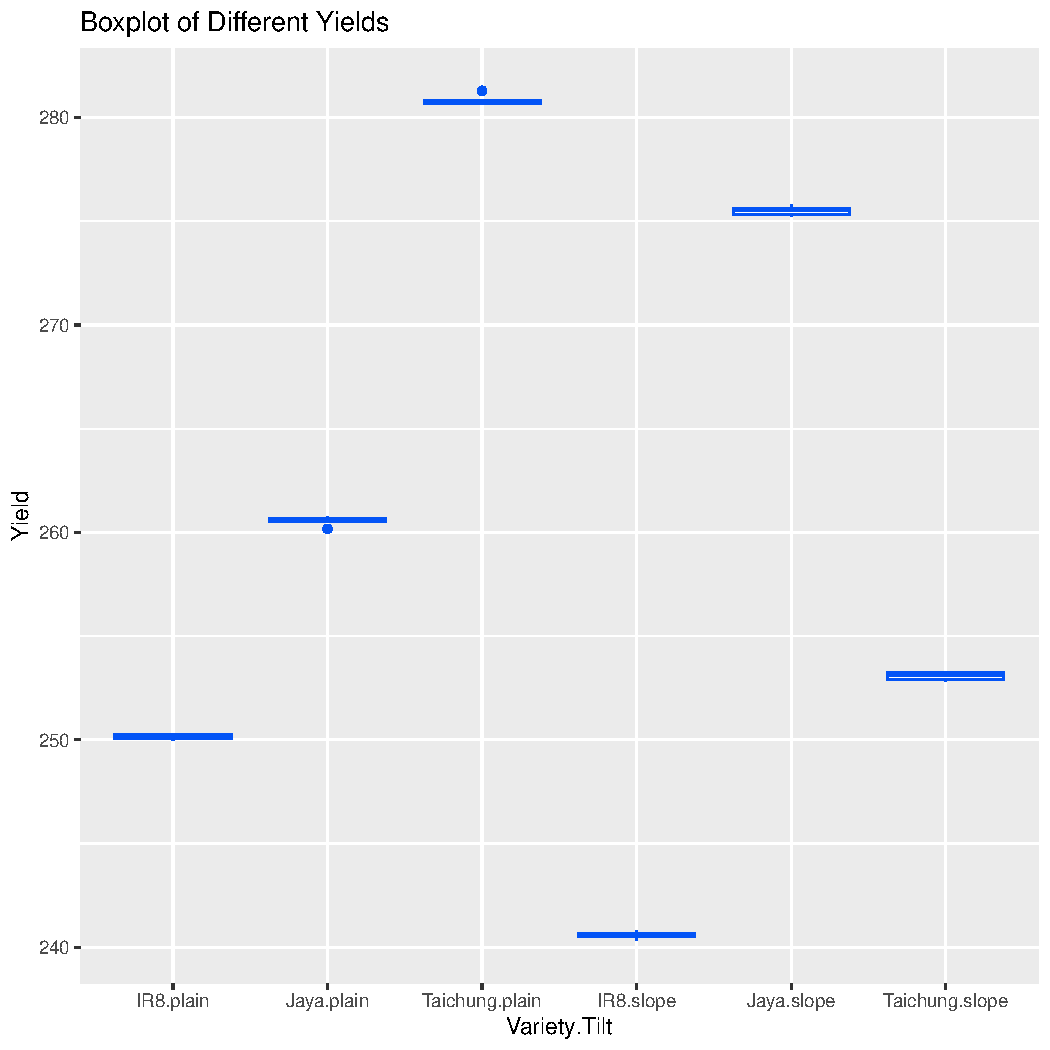
\includegraphics[width=\maxwidth]{figure/unnamed-chunk-17-1} 
\end{knitrout}

The boxplots verify that the homoscedasticity assumption is true and it also gives an idea about the interaction plot.

\newpage

\begin{knitrout}
\definecolor{shadecolor}{rgb}{0.969, 0.969, 0.969}\color{fgcolor}\begin{kframe}
\begin{alltt}
\hlkwd{with}\hlstd{(}\hlkwc{data} \hlstd{= paddy_data,} \hlkwd{interaction.plot}\hlstd{(tilt, variety, yield))}
\end{alltt}
\end{kframe}
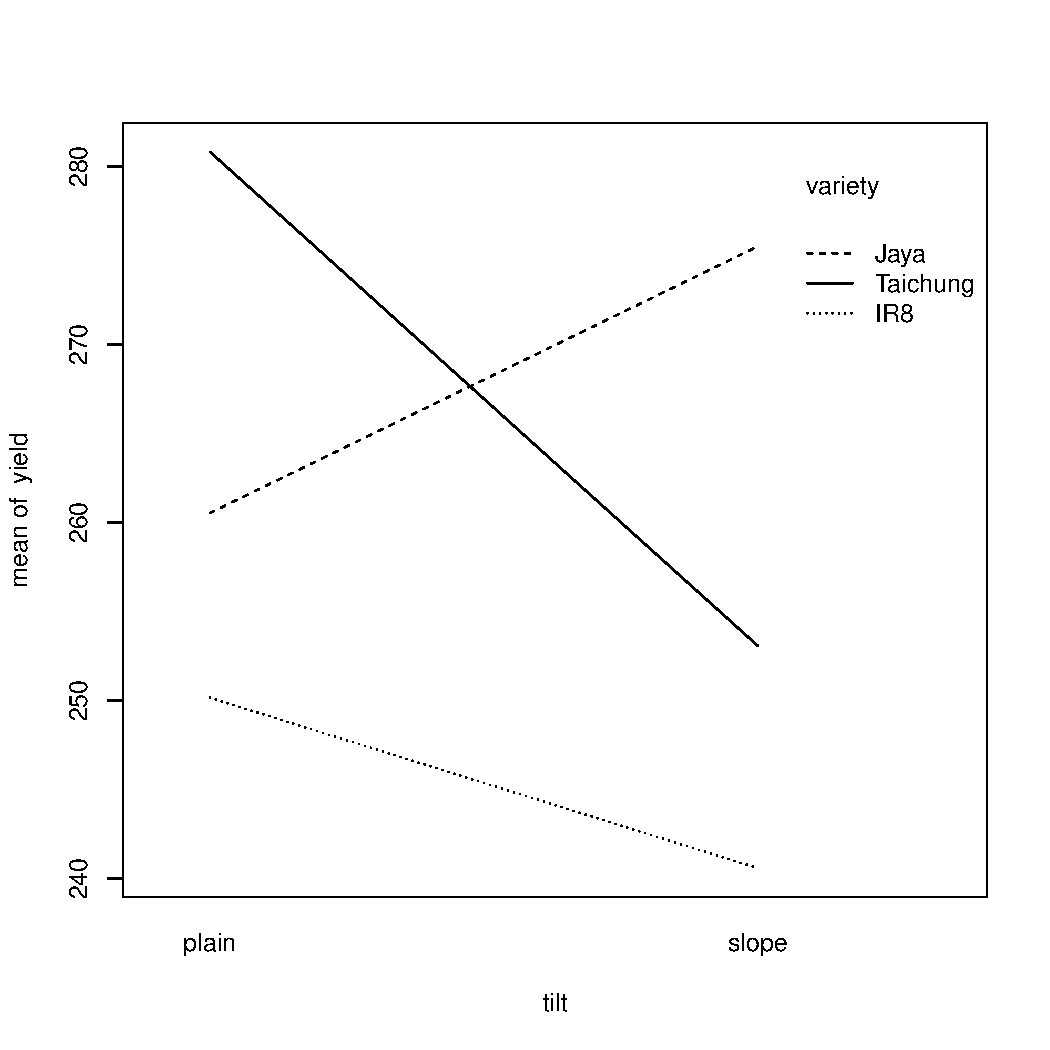
\includegraphics[width=\maxwidth]{figure/unnamed-chunk-18-1} 
\end{knitrout}

\newpage

\begin{knitrout}
\definecolor{shadecolor}{rgb}{0.969, 0.969, 0.969}\color{fgcolor}\begin{kframe}
\begin{alltt}
\hlstd{df2} \hlkwb{<-} \hlstd{paddy_data} \hlopt
  \hlkwd{group_by}\hlstd{(variety, tilt)} \hlopt
  \hlkwd{summarise}\hlstd{(}\hlkwc{mean_yield} \hlstd{=} \hlkwd{mean}\hlstd{(yield))}
\end{alltt}


{\ttfamily\noindent\itshape\color{messagecolor}{\#\# `summarise()` has grouped output by 'variety'. You can override using the\\\#\# `.groups` argument.}}\begin{alltt}
\hlstd{df2} \hlopt
  \hlkwd{ggplot}\hlstd{(}\hlkwd{aes}\hlstd{(}\hlkwc{x} \hlstd{= tilt,} \hlkwc{y} \hlstd{= mean_yield))} \hlopt{+}
  \hlkwd{geom_line}\hlstd{(}\hlkwd{aes}\hlstd{(}\hlkwc{group} \hlstd{= variety,} \hlkwc{color} \hlstd{= variety),} \hlkwc{linewidth} \hlstd{=} \hlnum{1.5}\hlstd{)} \hlopt{+}
  \hlkwd{geom_point}\hlstd{(}\hlkwd{aes}\hlstd{(}\hlkwc{color} \hlstd{= variety),} \hlkwc{size} \hlstd{=} \hlnum{4}\hlstd{)} \hlopt{+}
  \hlkwd{labs}\hlstd{(}\hlkwc{x} \hlstd{=} \hlstr{"Tilt"}\hlstd{,} \hlkwc{y} \hlstd{=} \hlstr{"Mean Yield"}\hlstd{,} \hlkwc{title} \hlstd{=} \hlstr{"Interaction Plot of Different Varieties"}\hlstd{)}
\end{alltt}
\end{kframe}
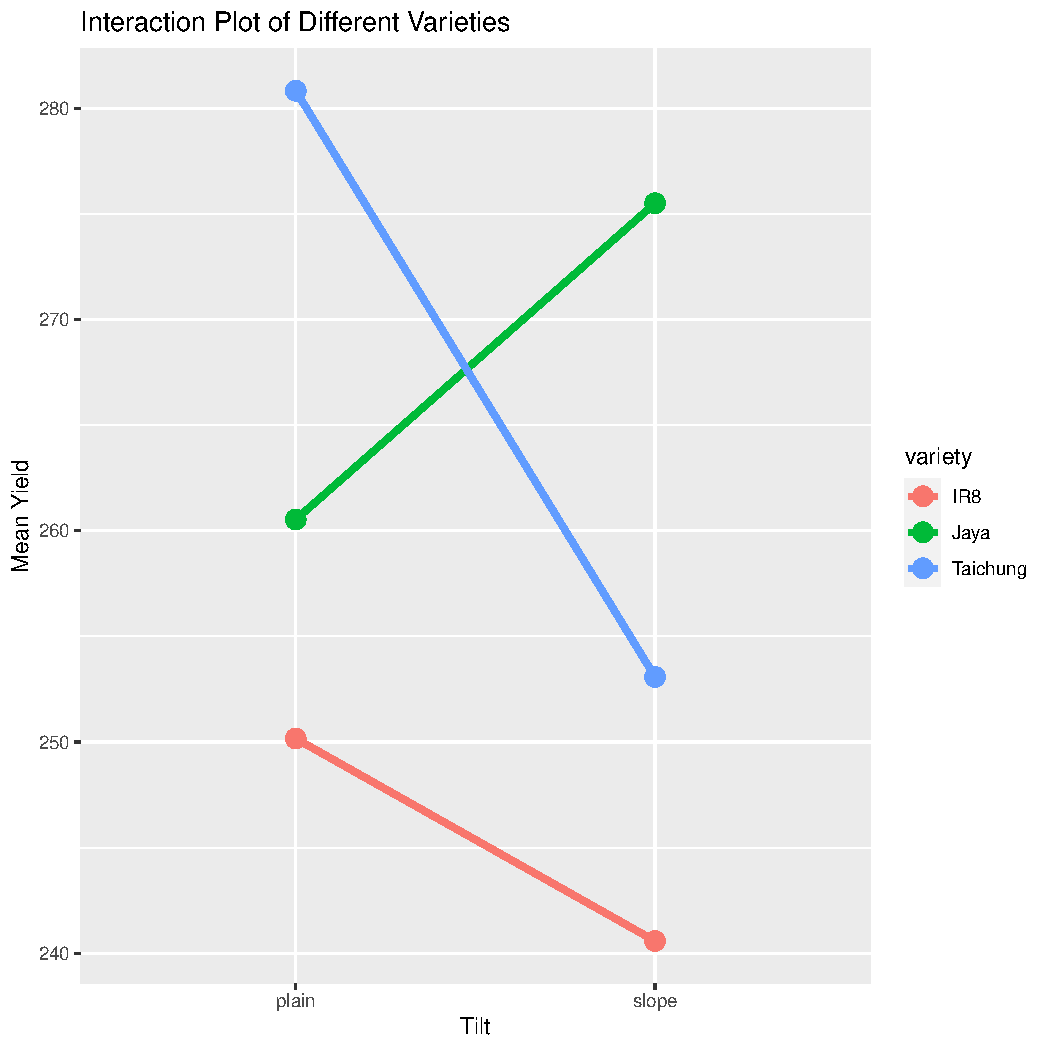
\includegraphics[width=\maxwidth]{figure/unnamed-chunk-19-1} 
\end{knitrout}

\begin{knitrout}
\definecolor{shadecolor}{rgb}{0.969, 0.969, 0.969}\color{fgcolor}\begin{kframe}
\begin{alltt}
\hlcom{# fit2 = lm(yield ~ variety + tilt + variety:tilt, data = paddy_data)}
\hlcom{# An abbrebriation of the above command is}
\hlstd{fit2} \hlkwb{=} \hlkwd{lm}\hlstd{(yield} \hlopt{~} \hlstd{variety}\hlopt{*}\hlstd{tilt,} \hlkwc{data} \hlstd{= paddy_data)}
\end{alltt}
\end{kframe}
\end{knitrout}

\begin{knitrout}
\definecolor{shadecolor}{rgb}{0.969, 0.969, 0.969}\color{fgcolor}\begin{kframe}
\begin{alltt}
\hlstd{fit2}
\end{alltt}
\begin{verbatim}
## 
## Call:
## lm(formula = yield ~ variety * tilt, data = paddy_data)
## 
## Coefficients:
##               (Intercept)                varietyJaya  
##                   250.162                     10.368  
##           varietyTaichung                  tiltslope  
##                    30.670                     -9.586  
##     varietyJaya:tiltslope  varietyTaichung:tiltslope  
##                    24.562                    -18.168
\end{verbatim}
\end{kframe}
\end{knitrout}

Here $\alpha_1$, $\beta_1$ have been forced to 0. \\

Also 2 of the 6 interaction terms $\gamma_{22}$ and $\gamma_{32}$ have been reported and others have been dropped.

\begin{knitrout}
\definecolor{shadecolor}{rgb}{0.969, 0.969, 0.969}\color{fgcolor}\begin{kframe}
\begin{alltt}
\hlkwd{model.matrix}\hlstd{(fit2)}
\end{alltt}
\begin{verbatim}
##    (Intercept) varietyJaya varietyTaichung tiltslope varietyJaya:tiltslope
## 1            1           0               0         0                     0
## 2            1           0               0         0                     0
## 3            1           0               0         0                     0
## 4            1           0               0         0                     0
## 5            1           0               0         0                     0
## 6            1           0               0         1                     0
## 7            1           0               0         1                     0
## 8            1           0               0         1                     0
## 9            1           0               0         1                     0
## 10           1           0               0         1                     0
## 11           1           1               0         0                     0
## 12           1           1               0         0                     0
## 13           1           1               0         0                     0
## 14           1           1               0         0                     0
## 15           1           1               0         0                     0
## 16           1           1               0         1                     1
## 17           1           1               0         1                     1
## 18           1           1               0         1                     1
## 19           1           1               0         1                     1
## 20           1           1               0         1                     1
## 21           1           0               1         0                     0
## 22           1           0               1         0                     0
## 23           1           0               1         0                     0
## 24           1           0               1         0                     0
## 25           1           0               1         0                     0
## 26           1           0               1         1                     0
## 27           1           0               1         1                     0
## 28           1           0               1         1                     0
## 29           1           0               1         1                     0
## 30           1           0               1         1                     0
##    varietyTaichung:tiltslope
## 1                          0
## 2                          0
## 3                          0
## 4                          0
## 5                          0
## 6                          0
## 7                          0
## 8                          0
## 9                          0
## 10                         0
## 11                         0
## 12                         0
## 13                         0
## 14                         0
## 15                         0
## 16                         0
## 17                         0
## 18                         0
## 19                         0
## 20                         0
## 21                         0
## 22                         0
## 23                         0
## 24                         0
## 25                         0
## 26                         1
## 27                         1
## 28                         1
## 29                         1
## 30                         1
## attr(,"assign")
## [1] 0 1 1 2 3 3
## attr(,"contrasts")
## attr(,"contrasts")$variety
## [1] "contr.treatment"
## 
## attr(,"contrasts")$tilt
## [1] "contr.treatment"
\end{verbatim}
\end{kframe}
\end{knitrout}

\begin{knitrout}
\definecolor{shadecolor}{rgb}{0.969, 0.969, 0.969}\color{fgcolor}\begin{kframe}
\begin{alltt}
\hlstd{fit2}\hlopt{$}\hlstd{rank}
\end{alltt}
\begin{verbatim}
## [1] 6
\end{verbatim}
\end{kframe}
\end{knitrout}

Observe that, when the rank of the model matrix is 6, R will report only 6 values in fit2.

\begin{knitrout}
\definecolor{shadecolor}{rgb}{0.969, 0.969, 0.969}\color{fgcolor}\begin{kframe}
\begin{alltt}
\hlkwd{summary}\hlstd{(fit2)}
\end{alltt}
\begin{verbatim}
## 
## Call:
## lm(formula = yield ~ variety * tilt, data = paddy_data)
## 
## Residuals:
##     Min      1Q  Median      3Q     Max 
## -0.3600 -0.1685  0.0360  0.1095  0.4580 
## 
## Coefficients:
##                            Estimate Std. Error t value Pr(>|t|)    
## (Intercept)               250.16200    0.09586 2609.68   <2e-16 ***
## varietyJaya                10.36800    0.13557   76.48   <2e-16 ***
## varietyTaichung            30.67000    0.13557  226.24   <2e-16 ***
## tiltslope                  -9.58600    0.13557  -70.71   <2e-16 ***
## varietyJaya:tiltslope      24.56200    0.19172  128.12   <2e-16 ***
## varietyTaichung:tiltslope -18.16800    0.19172  -94.76   <2e-16 ***
## ---
## Signif. codes:  0 '***' 0.001 '**' 0.01 '*' 0.05 '.' 0.1 ' ' 1
## 
## Residual standard error: 0.2143 on 24 degrees of freedom
## Multiple R-squared:  0.9998,	Adjusted R-squared:  0.9998 
## F-statistic: 2.604e+04 on 5 and 24 DF,  p-value: < 2.2e-16
\end{verbatim}
\end{kframe}
\end{knitrout}

\newpage

\begin{knitrout}
\definecolor{shadecolor}{rgb}{0.969, 0.969, 0.969}\color{fgcolor}\begin{kframe}
\begin{alltt}
\hlstd{df3} \hlkwb{<-} \hlkwd{data.frame}\hlstd{(fit2}\hlopt{$}\hlstd{residuals)}

\hlstd{df3} \hlopt
  \hlkwd{ggplot}\hlstd{(}\hlkwd{aes}\hlstd{(}\hlkwc{x} \hlstd{=} \hlnum{1}\hlopt{:}\hlkwd{length}\hlstd{(fit2.residuals),} \hlkwc{y} \hlstd{= fit2.residuals))} \hlopt{+}
  \hlkwd{geom_point}\hlstd{(}\hlkwc{color} \hlstd{=} \hlstr{"red"}\hlstd{,} \hlkwc{size} \hlstd{=} \hlnum{3}\hlstd{)} \hlopt{+}
  \hlkwd{geom_hline}\hlstd{(}\hlkwc{yintercept} \hlstd{=} \hlnum{0}\hlstd{,} \hlkwc{color} \hlstd{=} \hlstr{"blue"}\hlstd{,} \hlkwc{linewidth} \hlstd{=} \hlnum{1.5}\hlstd{)} \hlopt{+}
  \hlkwd{labs}\hlstd{(}\hlkwc{x} \hlstd{=} \hlstr{"Index"}\hlstd{,} \hlkwc{y} \hlstd{=} \hlstr{"Residuals"}\hlstd{,} \hlkwc{title} \hlstd{=} \hlstr{"Residuals of fit2"}\hlstd{)}
\end{alltt}
\end{kframe}
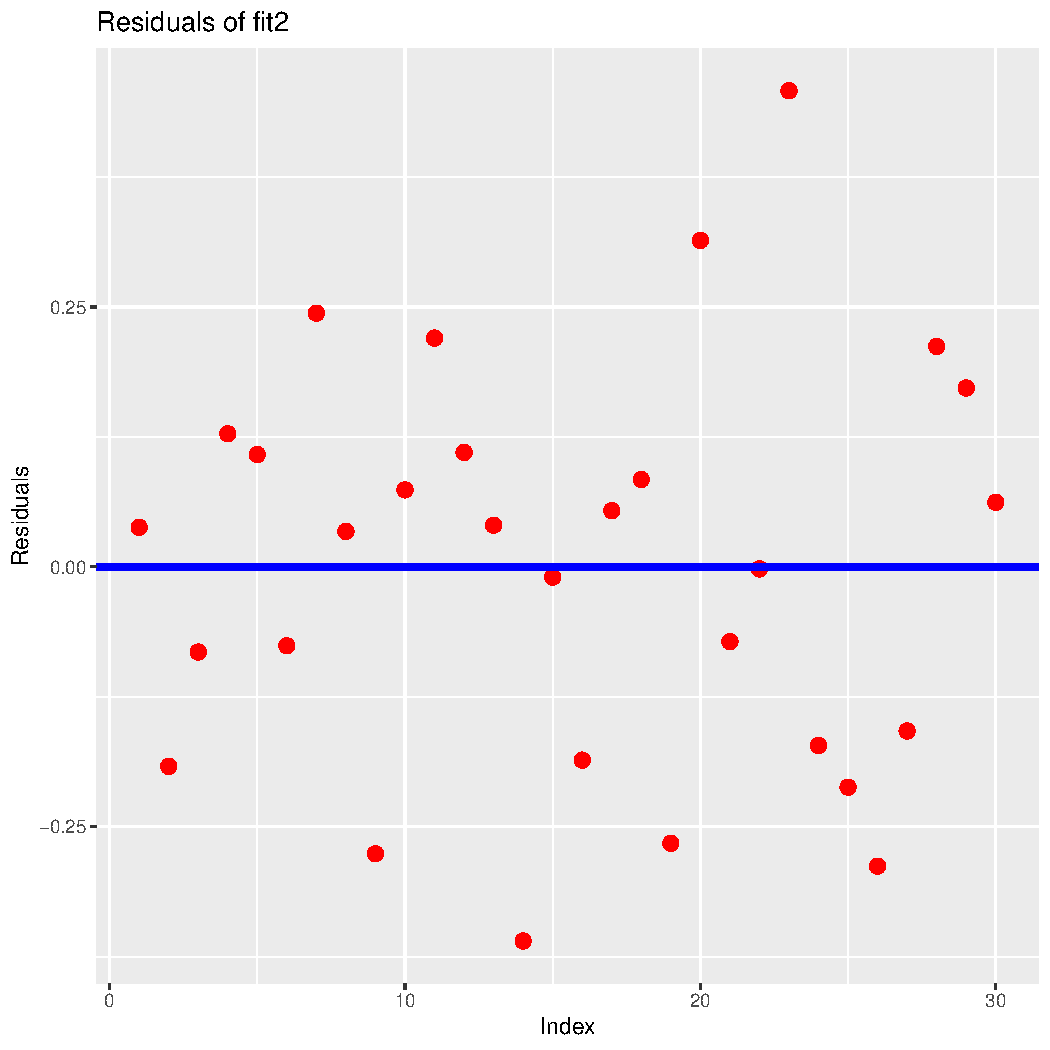
\includegraphics[width=\maxwidth]{figure/unnamed-chunk-25-1} 
\end{knitrout}






\end{document}
